\documentclass[tikz,border=8pt]{standalone}
\usepackage{pgfplots}
\pgfplotsset{compat=1.18}
\usepgfplotslibrary{groupplots}
\usetikzlibrary{arrows.meta,positioning}
\definecolor{chapterteal}{HTML}{196F6B}
\definecolor{chapterrust}{HTML}{A3472F}
\definecolor{chaptergold}{HTML}{C58B18}
\definecolor{chapterblue}{HTML}{174F75}

\begin{document}

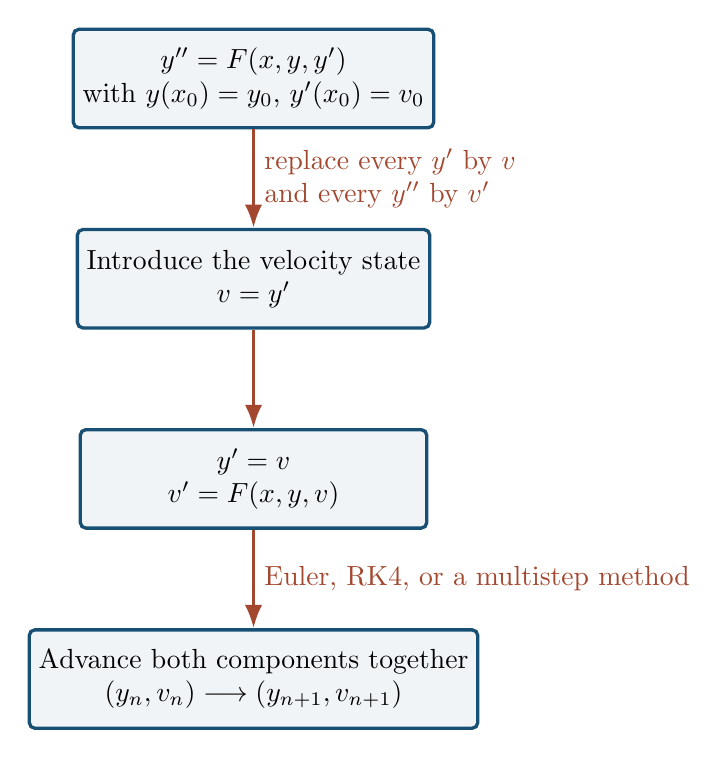
\begin{tikzpicture}[
  >=Latex,
  node distance=1.25cm,
  box/.style={
    draw=chapterblue,
    very thick,
    fill=chapterblue!6,
    rounded corners=2pt,
    align=center,
    minimum width=4.4cm,
    minimum height=1.25cm
  },
  arrow/.style={->,very thick,chapterrust}
]
  \node[box] (second) {$y''=F(x,y,y')$\\with $y(x_0)=y_0$, $y'(x_0)=v_0$};
  \node[box,below=of second] (define) {Introduce the velocity state\\$v=y'$};
  \node[box,below=of define] (system) {$y'=v$\\$v'=F(x,y,v)$};
  \node[box,below=of system] (advance) {Advance both components together\\$(y_n,v_n)\longrightarrow(y_{n+1},v_{n+1})$};

  \draw[arrow] (second) -- node[right,align=left] {replace every $y'$ by $v$\\and every $y''$ by $v'$} (define);
  \draw[arrow] (define) -- (system);
  \draw[arrow] (system) -- node[right] {Euler, RK4, or a multistep method} (advance);
\end{tikzpicture}

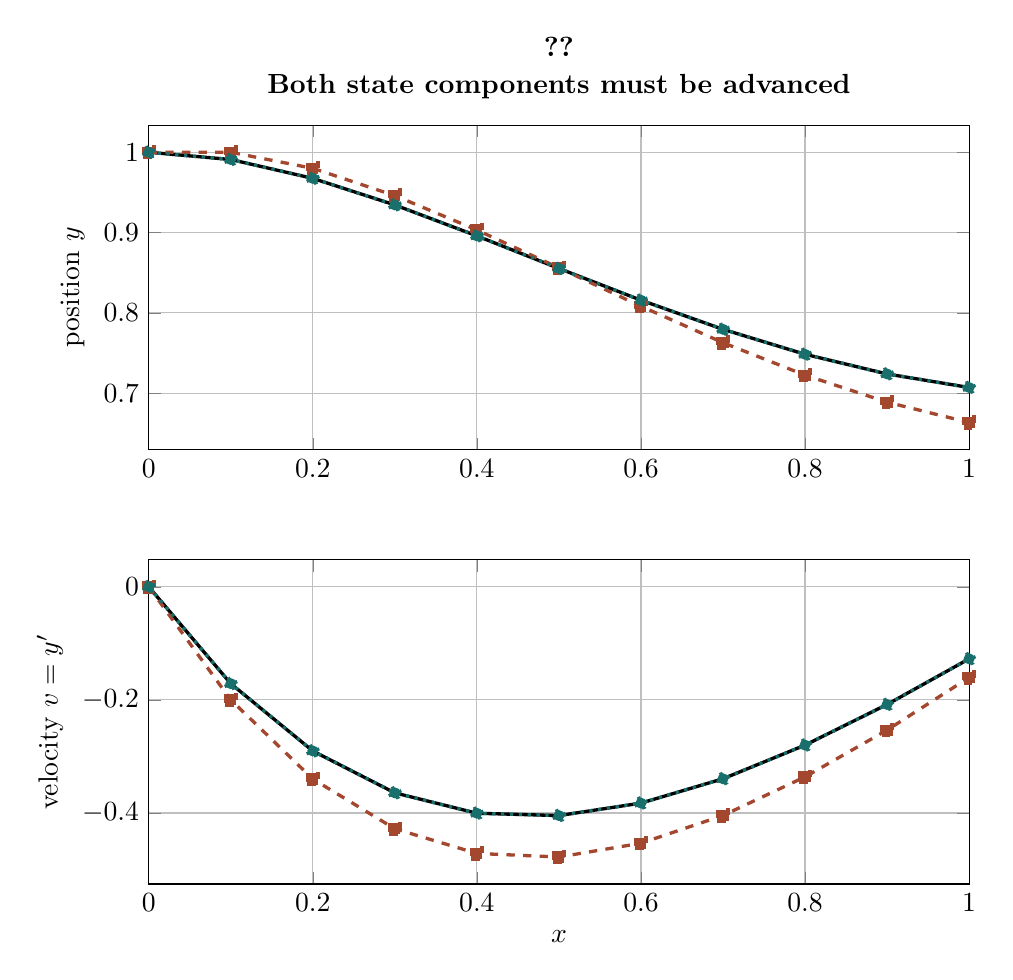
\begin{tikzpicture}
\begin{groupplot}[
  group style={group size=1 by 2,vertical sep=1.4cm},
  width=12cm,
  height=5.7cm,
  xmin=0,xmax=1,
  xtick={0,0.2,0.4,0.6,0.8,1},
  grid=both,
  legend columns=3,
  legend style={font=\small,at={(0.5,1.05)},anchor=south,draw=none},
  every mark/.append style={scale=0.75}
]
\nextgroupplot[
  ylabel={position $y$},
  title={Both state components must be advanced},
  title style={font=\bfseries},
  legend to name=statelegend
]
\addplot[black,very thick] coordinates {
  (0,1) (.1,.990967011) (.2,.967477986) (.3,.934388110)
  (.4,.895846217) (.5,.855347749) (.6,.815789938) (.7,.779527816)
  (.8,.748429877) (.9,.723932462) (1,.707092096)
};
\addlegendentry{exact}
\addplot[chapterrust,very thick,dashed,mark=square*] coordinates {
  (0,1) (.1,1) (.2,.98) (.3,.946) (.4,.9032) (.5,.85604)
  (.6,.808248) (.7,.7628936) (.8,.72244512) (.9,.688828464) (1,.663486237)
};
\addlegendentry{Euler}
\addplot[chapterteal,very thick,dotted,mark=*] coordinates {
  (0,1) (.1,.990966667) (.2,.967477189) (.3,.934386804)
  (.4,.895844387) (.5,.855345410) (.6,.815787133) (.7,.779524604)
  (.8,.748426329) (.9,.723928656) (1,.707088113)
};
\addlegendentry{RK4}

\nextgroupplot[
  xlabel={$x$},
  ylabel={velocity $v=y'$}
]
\addplot[black,very thick] coordinates {
  (0,0) (.1,-.171316033) (.2,-.290380720) (.3,-.364510939)
  (.4,-.400510411) (.5,-.404639595) (.6,-.382600868) (.7,-.339536498)
  (.8,-.280037112) (.9,-.208158619) (1,-.127445737)
};
\addplot[chapterrust,very thick,dashed,mark=square*] coordinates {
  (0,0) (.1,-.2) (.2,-.34) (.3,-.428) (.4,-.4716) (.5,-.47792)
  (.6,-.453544) (.7,-.4044848) (.8,-.33616656) (.9,-.253422272) (1,-.160503510)
};
\addplot[chapterteal,very thick,dotted,mark=*] coordinates {
  (0,0) (.1,-.171316667) (.2,-.290381622) (.3,-.364511820)
  (.4,-.400511048) (.5,-.404639827) (.6,-.382600586) (.7,-.339535640)
  (.8,-.280035655) (.9,-.208156570) (1,-.127443130)
};
\end{groupplot}
\node at ($(group c1r1.north)+(0,1.0cm)$) {\ref{statelegend}};
\end{tikzpicture}

\end{document}
